\chapter{Konzeptentwurf}
\label{cha:vorgehen}

Dieses Kapitel beschreibt die methodische Herleitung eines technischen Konzepts zur Umsetzung des in Kapitel~\ref{cha:Grundlagen} vorgestellten Systems. Basierend auf den identifizierten technologischen Grundlagen erfolgt zunächst eine strukturierte Analyse der funktionalen und nicht-funktionalen Anforderungen mithilfe des Requirements Engineerings.

Auf dieser Grundlage werden mehrere Lösungsoptionen konzipiert, die für den Einsatz unterschiedlicher Hardwarekomponenten geeignet sind. Ein wesentlicher Bestandteil des Konzepts ist der Systementwurf. In diesem wird die Architektur der miteineinander interagierenden Hardwarekomponenten beschrieben. Außerdem wird erklärt mit welchen Software-Bibliotheken gearbeitet wurde und wie die Informationen im Speicher der NFC-Tags organisiert ist.

Ziel ist es, eine nachvollziehbare und belastbare Begründung für die gewählte Vorgehensweise zu liefern, die die Anforderungen der Anwendung erfüllt und eine verlässliche Grundlage für die anschließende Umsetzung bietet.

\section{Anforderungsanalyse mittels Requirements Engineering}
\label{sec:anforderungsanalyse}

Im Rahmen dieser Arbeit bildet das Requirements Engineering die methodische Basis für die Konzeption eines funktionalen und technisch realisierbaren Systems. Dabei werden sowohl funktionale als auch nicht-funktionale Anforderungen betrachtet. Die gewonnenen Erkenntnisse dienen anschließend als Ausgangspunkt für den Systementwurf und die Auswahl geeigneter technischer Komponenten.

\subsection{Funktionale Anforderungen}

Um die Anforderungen an das zu entwickelnde System bestimmen zu können, soll zunächst die Funktionalität aus der Sicht des Anwenders in Anforderungen festgehalten werden.

\begin{table}[H]
	\centering
	\caption{funktionale Systemanforderungen}
	\label{tab:f_anforderungen}
	\begin{tabular}{|p{0.075\linewidth}|p{0.75\linewidth}|}
		\hline
		\textbf{ID} & \textbf{Anforderung} \\ \hline
		
		F01 & Der Anwender soll Produkte auf einer Fertigungskette mittels einer eindeutigen und einmaligen Identifikationsnummer identifizieren können. \\ \hline
		F02 & Der Anwender soll über die Position und den Zustand der Produkte auf dem Bandumlaufsystem informiert werden können. \\ \hline
		F03 & Die Positionen und Zustände der Produkte sollen visuell dargestellt werden. \\ \hline
		F04 & Das Bandumlaufsystem soll basierend auf den Produktzuständen gesteuert werden können. \\ \hline
		F05 & Die Produkte sollen einen NFC-Tag mit allen relevanten Zustandsinformationen und der eindeutigen Identifikationsnummer tragen. \\ \hline
		F06 & Über vier NFC-Lesegeräte sollen die Position und die Zustände der Produkte ermittelt und geschrieben werden können. \\ \hline
		F07 & Die NFC-Lesegeräte müssen ein Verweilen eines Produktes an einer Station erkennen können. \\ \hline
		F08 & Das Tracking-System soll den letzten Zustand eines Produktes speichern. \\ \hline
		F09 & Die Speicherung von Zuständen soll auf den NFC-Tags und im System erfolgen. \\ \hline
	\end{tabular}
\end{table}


\subsection{Nicht funktionale Anforderungen}

Nachdem die Funktion des Systems ermittelt wurde, sollen entsprechende technische, nicht funktionale Anforderungen festgehalten werden. 

\begin{table}[H]
	\centering
	\caption{nicht-funktionale Systemanforderungen}
	\label{tab:nf_anforderungen}
	\begin{tabular}{|p{0.075\linewidth}|p{0.75\linewidth}|}
		\hline
		\textbf{ID} & \textbf{Anforderung} \\ \hline

		NF01 & Die Kommunikation von Informationen von und zu den NFC-Lesegeräten soll über ein leichtgewichtiges Netzwerkprotokoll erfolgen. \\ \hline
		NF02 & Die Netzwerkkommunikation sollte drahtlos funktionieren. \\ \hline
		NF03 & MQTT-Nachrichten können mit einer Quality-of-Service-Stufe 0 gesendet werden. \\ \hline
		NF04 & Die Software der Mikrocontroller soll generisch aufgebaut sein und logische Erweiterungen ermöglichen. \\ \hline
		NF05 & Diskrepanzen von Zuständen im System und auf den Tags dürfen nicht entstehen. Eine Behandlung des Problems muss in Software abgebildet werden. \\ \hline
		NF06 & Das Tracking-System soll über eine Anbindung zu einer SPS verfügen. \\ \hline
		NF07 & Das Bandumlaufsystem soll weiterhin über die bestehende SPS gesteuert werden. \\ \hline
		NF08 & Node-Red soll als Visualisierungssoftware verwendet werden. \\ \hline
	\end{tabular}
\end{table}



\section{Hardwarebewertung mithilfe der Nutzwertanalyse}
\label{sec:hardwarebewertung}
Die zur Auswahl nötige Bewertung der Hardware soll basierend auf einer Nutzwertanalyse passieren. Drei verschiedene Hardwareklassen sollen betrachtet werden, um den Systemebenen Hardwarekomponenten zuweisen zu können. Dazu gehören die NFC-Tags, die NFC-Lesegeräte und die Controller-Einheiten. 

\subsection{NFC-Tags}
NFC-Tags unterscheiden sich im Hinblick auf unterschiedliche Faktoren. Dazu zählen beispielsweise: Speicherkapazität,  Form und Größe. Das NFC Forum definiert fünf Tag-Typen (Typ 1 bis Typ 5), die auf existierenden RFID-Technologien basieren [\autoref{tab:nfc_typen}]. 

\begin{table}[H]
	\centering
	\caption{Vergleich der NFC-Tag-Typen gemäß NFC Forum \cite{nfcforum2024}}
	\label{tab:nfc_typen}
	\begin{tabular}{|p{0.075\linewidth}|p{0.18\linewidth}|p{0.12\linewidth}|p{0.12\linewidth}|p{0.18\linewidth}|p{0.25\linewidth}|}
		\hline
		\textbf{Tag-Typ} & \textbf{Technologie-Basis} & \textbf{Speicher} & \textbf{Datenrate} & \textbf{Sicherheit} & \textbf{Besonderheiten} \\
		\hline
		Typ 1 & Innovision Topaz & 96B – 2KB & 106kbit/s & Keine Authentifizierung & Kostengünstig, einfache Anwendungen \\
		Typ 2 & NXP MIFARE Ultralight und NTAG & bis 2KB & 106kbit/s & Einfach & Häufig in Tickets, Werbeanwendungen \\
		Typ 3 & Sony FeliCa & bis 1MB & 212–424 kbit/s & Zugriffskontrolle möglich & Hohe Geschwindigkeit, verbreitet in Japan \\
		Typ 4 & NXP DESFire, Smartcard & bis 32KB+ & 106–424 kbit/s & Hohe Sicherheit (AES, ISO 7816) & Zutrittssysteme, sichere Speicherung \\
		Typ 5 & ST25, NXP ICODE (ISO 15693) & bis ca. 64KB & bis 53kbit/s & Variabel & Größere Reichweite, Industrieeinsatz \\
		\hline
	\end{tabular}
\end{table}

Basierend auf gegebenen Informationen zu den Tag-Typen wurde die Nutzwertanalayse durchgeführt. Die Eigenschaften wurden entsprechend als Bewertungskriterien gewichtet, wodurch nach zusammenzählen der vergebenen Punkte der passende Tag-Typ und aus \ref{tab:nfc_typen} das passende Produkt ermittelt werden konnte. 

Die höchste Gewichtung hat in der Analyse die Lesegeschwindigkeit erhalten, da am Bandumlaufsystem eine Verarbeitung von Informationen in Echtzeit relevant ist. Das folgt daraus, dass der Zustand eines Produktes an einer Station ermittelt und dann auf den Tag geschrieben werden muss [\ref{tab:nutzwertanalyse-nfc-tags}].

\begin{table}[H]
	\centering
	\caption{Nutzwertanalyse zur Bewertung von NFC-Tag-Typen (1 - 5, wobei 5: sehr gut}
	\label{tab:nutzwertanalyse-nfc-tags}
	\begin{tabular}{|l|c|c|c|c|c|c|}
		\hline
		\textbf{Kriterium} & \textbf{Gewichtung} & \textbf{Typ 1} & \textbf{Typ 2} & \textbf{Typ 3} & \textbf{Typ 4} & \textbf{Typ 5} \\ \hline
		Lesegeschwindigkeit         & 25\% & 2 & 3 & 2 & 4 & 5 \\ \hline
		Speicherkapazität           & 20\% & 2 & 3 & 4 & 5 & 4 \\ \hline
		Kosten                      & 20\% & 5 & 4 & 3 & 2 & 3 \\ \hline
		Kompatibilität              & 15\% & 3 & 4 & 2 & 5 & 4 \\ \hline
		Energieeffizienz (passiv)   & 10\% & 5 & 5 & 4 & 3 & 4 \\ \hline
		Verfügbarkeit am Markt      & 10\% & 3 & 5 & 2 & 4 & 4 \\ \hline
		\textbf{Gesamtnutzwert}     &      & \textbf{3.10} & \textbf{4.00} & \textbf{2.85} & \textbf{4.00} & \textbf{4.10} \\ \hline
	\end{tabular}
\end{table}

Tag Typ 2 ist nach dieser Analyse der favorisierte Typ. Für die Arbeit wurde entsprechend ein NXP NTAG213-Tag gewählt. Dieser bietet einen EEPROM-Speicher von 144 Bytes, der in 4 Byte große Seiten (Pages) unterteilt ist. Daraus ergeben sich 36 adressierbare Blöcke. Von diesen sind laut Datenblatt etwa 112 Bytes frei vom Anwender beschreibbar \cite{nxp_ntag213f_datasheet}, da einige Speicherbereiche für Systemfunktionen wie die UID, Konfiguration und Sicherheitsmechanismen reserviert sind. Das genügt für das Schreiben von binärcodierten Zuständen und Tracking-Positionen auf den Tag. Entsprechend wurde eine Codierungstabelle in \autoref{sec:systementwurf} ausgearbeitet. 

\subsection{NFC-Lesegeräte}

Da nach der Auswahl des NFC-Tags eine entsprechende Kompatibilität gewährleistet sein muss, reduziert sich die Vielfalt an geeigneten Lesegeräten. Aus diesem Grund wurde auf eine detaillierte Nutzwertanalyse verzichtet, da es sich nicht um gleichwertig vergleichbare Alternativen handelt, sondern primär um die Auswahl eines technisch kompatiblen und verfügbaren Bauteils.

Insbesondere muss das NFC-Lesegerät den Frequenzbereich von 13{,}56\,MHz unterstützen und mit ISO/IEC 14443 Typ~A kompatibel sein, um mit dem gewählten NTAG213-Tag kommunizieren zu können. Zusätzlich waren Kriterien wie Verfügbarkeit, Preis und Schnittstellenunterstützung entscheidend.

Der PN532 von NXP hat sich als geeignete Wahl erwiesen. Das Modul unterstützt sowohl I\textsuperscript{2}C (Inter Integrated Circuit) als auch SPI als Kommunikationsschnittstelle und bietet eine effektive Reichweite von ca. 5–10\,cm. Diese ist für das vorliegende System ausreichend, da die Produkte gezielt an den Sensorstationen positioniert werden und dort die Datenübertragung stattfindet.

Als bevorzugte Schnittstelle zwischen Mikrocontroller und NFC-Modul wurde SPI gewählt, da sie gegenüber I\textsuperscript{2}C eine höhere Datenrate, robustere Signalübertragung und eine bessere Unterstützung bei Echtzeitanforderungen bietet.


\subsection{Controller-Einheiten}

\begin{table}[H]
	\centering
	\caption{Nutzwertanalyse zur Bewertung der Mikrocontroller(1 - 5, wobei 5: sehr gut)}
	\label{tab:nwa_ctrl}
	\begin{tabular}{|l|c|c|c|}
		\hline
		\textbf{Kriterium} & \textbf{Gewichtung} & \textbf{ESP8266} & \textbf{ESP32} \\ \hline
		Rechenleistung          & 20\% & 3 & 5 \\ \hline
		Energieverbrauch        & 25\% & 4 & 3 \\ \hline
 		GPIO-Pins				& 15\% & 3 & 5 \\ \hline
		kabellos netzwerkfähig	& 20\% & 5 & 5 \\ \hline
		Preis                   & 20\% & 5 & 4 \\ \hline
		\textbf{Gesamtnutzwert} &       & \textbf{4,05} & \textbf{4,3} \\ \hline
	\end{tabular}
\end{table}

Die Nutzwertanalyse wurde auf zwei Mikrocontroller eingegrenzt: den ESP8266 und den ESP32. Beide Module bieten eine solide Grundlage zur Implementierung von Anwendungen mit geringer bis mittlerer Komplexität, verfügen über integrierte Netzwerkschnittstellen, sind breit verfügbar und gut dokumentiert (vgl. Tabelle~\ref{tab:nwa_ctrl}). Aufgrund dieser Gemeinsamkeiten wurde auf die Einbeziehung weiterer Hardwarevarianten verzichtet.

Das Ergebnis der Analyse zeigt, dass der ESP32 insgesamt eine höhere Nutzwertpunktzahl erreicht. Dennoch fiel die Entscheidung in diesem Projekt zugunsten des ESP8266 aus, da einige der Stärken des ESP32 für den vorliegenden Anwendungsfall nicht ausschlaggebend sind.

So verfügt der ESP32 über zwei CPU-Kerne, wodurch parallele Prozesse (Multithreading) möglich werden. Dies kann bei gleichzeitiger Verarbeitung von Kommunikations- und Steuerungsaufgaben vorteilhaft sein. Im betrachteten System ist jedoch eine sequenzielle Verarbeitung – etwa durch Interrupt-gesteuerte Abläufe – ausreichend, da beispielsweise das Schreiben auf einen NFC-Tag erst nach vollständigem Empfang der Nachricht über MQTT erfolgt. Somit ergibt sich hier kein zwingender Vorteil für die Mehrkernarchitektur.

Ein weiterer Unterschied besteht in der Anzahl der verfügbaren GPIO-Pins: Der ESP32 bietet mehr konfigurierbare Pins, was insbesondere bei komplexeren Schaltungen hilfreich sein kann. Beim ESP8266 hingegen kam es im Testbetrieb vereinzelt zu Einschränkungen aufgrund mehrfach belegter Pins. Beispielsweise musste das Slave-Select-Signal des SPI-Busses auf einen alternativen Pin gelegt werden, da die ursprüngliche Konfiguration den Flash-Vorgang blockierte. Dennoch stehen auch beim ESP8266 ausreichend Pins zur Verfügung, um die Anforderungen dieses Projekts zuverlässig zu erfüllen.

Hinsichtlich Energieverbrauch und Preis schneidet der ESP8266 besser ab. Diese Vorteile sind auf den geringeren Systemumfang und die reduzierte Hardwarekomplexität zurückzuführen – ein relevantes Kriterium für ressourcenschonende Embedded-Anwendungen. Insgesamt erfüllt der ESP8266 damit alle funktionalen Anforderungen des Systems und stellt eine technisch sinnvolle Wahl dar, um mit dem NFC-Lesegerät zu kommunizieren. Der ESP32 wäre jedoch ebenfalls eine geeignete Alternative mit erweiterter Funktionalität für zukünftige Skalierungen.

\subsection{Zentraleinheit: Raspberry Pi}


Für die zentrale Verarbeitung und Weiterleitung der MQTT-Nachrichten wurde ein Raspberry Pi 3B+ als Systemzentrale eingesetzt. Dieses Gerät erfüllt die Anforderungen an eine kontinuierliche Betriebsbereitschaft, stabile Netzwerkkommunikation und eine ausreichende Rechenleistung für die Verwaltung eines erhöhten Nachrichtendurchsatzes. 

Eine Einbeziehung des Raspberry Pi in die zuvor dargestellte Nutzwertanalyse der Mikrocontroller erfolgte bewusst nicht, da er auf einer übergeordneten Systemebene agiert. Während die Mikrocontroller-Einheiten an den Stationen in direktem Kontakt mit den Sensoren stehen und deren Steuerung übernehmen, fungiert der Raspberry Pi als dedizierte Zentraleinheit zur Aggregation und Verteilung der Systemdaten über das MQTT-Protokoll.

Aufgrund der ausgezeichneten Softwareunterstützung, der nativen Kompatibilität mit MQTT-Broker-Implementierungen (z.~B. Mosquitto) sowie der Möglichkeit zur einfachen Netzwerk- und Systemintegration wurde auf eine vergleichende Analyse alternativer Hardwareplattformen verzichtet. Der Raspberry Pi stellte hier eine erprobte und funktional bewährte Lösung dar.

\subsection{Gesamtkostenanalyse}
\label{sec:gesamtkostenanalyse}

\autoref{tab:kostenanalyse} zeigt die Gesamtkostenübersicht aller im Projekt eingesetzten Hardwarekomponenten. Es wurden jeweils übliche Preise von Amazon herangezogen (Stand: Mai 2025). Die Preise verstehen sich als Stückpreise und beinhalten keine Mengenrabatte oder Versandkosten.

\begin{table}[H]
	\centering
	\caption{Gesamtkostenanalyse der verwendeten Hardware}
	\label{tab:kostenanalyse}
	\begin{tabular}{|p{0.4\linewidth}|c|c|c|}
		\hline
		\textbf{Komponente} & \textbf{Anzahl} & \textbf{Einzelpreis [€]} & \textbf{Gesamtpreis [€]} \\
		\hline
		NFC-Tag (NTAG213-Set) & 60 & 0{,}13 & 8{,}00 \\
		NFC-Lesegerät (PN532 Modul) & 4 & 7{,}00 & 28{,}00 \\
		Mikrocontroller (ESP8266) & 4 & 3{,}50 & 21{,}00 \\
		Raspberry Pi 3B+ & 1 & 67{,}00 & 67{,}00 \\
		Jumperwires & 1 & 7{,}00 & 7{,}00 \\
		Spannungsversorgung (Netzteil) & 4 & 1{,}75 & 7{,}00 \\
		USB-Kabel & 4 & 1{,}75 & 7{,}00 \\
		\hline
		\textbf{Gesamtkosten} & & & \textbf{145{,}00} \\
		\hline
	\end{tabular}
\end{table}

Die Gesamtkosten belaufen sich auf ca. \textbf{145,00€} für ein vollständiges Testsystem mit vier Stationen und einer zentralen Steuereinheit. Bei einer Skalierung auf weitere Stationen würden die Kosten für die zusätzlichen ESP8266-Controller, NFC-Lesegeräte, Kabel und Netzteile anfallen. Ein einzelner zusätzlicher Stationsknoten verursacht dabei geschätzte Mehrkosten von etwa \textbf{14,00€} (PN532 + ESP8266 + Spannungsversorgung + USB Kabel).

\section{Systementwurf}
\label{sec:systementwurf}

\subsection{Organisation der Hardwarekomponenten}
\begin{figure}[H] % [H] nur mit \usepackage{float}
	\centering
	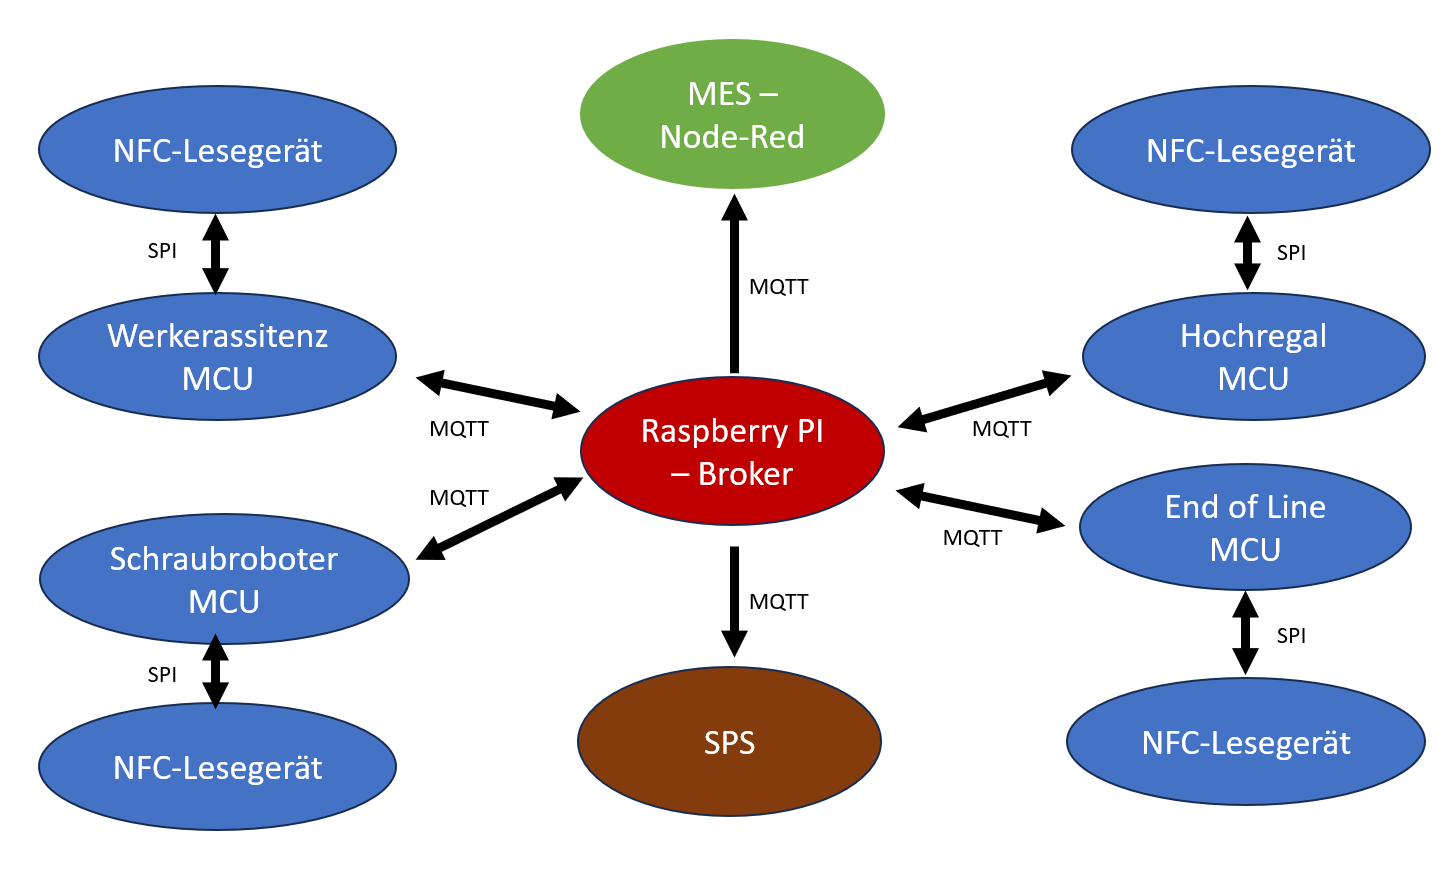
\includegraphics[width=0.8\textwidth]{images/Systemarchitektur.png}
	\caption{Systemarchitektur des NFC-Tracking-Systems (MCU: Microcontroller Unit --> ESP8266)}
	\label{fig:systemarchitektur}
\end{figure}

Die Hardwarekomponenten des Systems sind entsprechend der in Abbildung \ref{fig:systemarchitektur} dargestellten Architektur organisiert. Ab den Mikrocontrollern erfolgt der Informationsaustausch über das MQTT-Protokoll (vgl. Abschnitt \autoref{sec:mqtt}). Die ESP8266-Mikrocontroller sind über das SPI-Protokoll (Serial Peripheral Interface, vgl. \autoref{sec:spi}) mit den jeweiligen NFC-Lesegeräten (vgl. \autoref{sec:nfc}) verbunden und kommunizieren anschließend drahtlos mit dem zentralen Raspberry Pi.

Der Raspberry Pi fungiert als zentrale Einheit und ist ebenfalls drahtlos mit der speicherprogrammierbaren Steuerung (SPS, vgl. \autoref{sec:sps}) sowie mit dem MES-System (Manufacturing Execution System, vgl. \autoref{sec:mes}) verbunden. Das MES-System setzt sich in dieser Projektbeschreibung ausschließlich aus dem Node-Red-Dashboard zusammen, beinhaltet aber noch weitere Systemkomponenten. 

\subsection{Speicherorganisation der NFC-Tags}

\begin{table}[H]
	\centering
	\caption{Mögliche Zustände im Tracking-Block}
	\label{tab:tracking_states}
	\begin{tabular}{|c|l|}
		\hline
		\textbf{Hex-Wert} & \textbf{Zustand} \\ \hline
		0x01 & to\_shelf \\ \hline
		0x02 & at\_shelf \\ \hline
		0x03 & in\_shelf \\ \hline
		0x04 & to\_screwing \\ \hline
		0x05 & at\_screwing \\ \hline
		0x06 & to\_eol \\ \hline
		0x07 & at\_eol \\ \hline
		0x08 & at\_assembling \\ \hline
		0x09 & to\_assembling \\ \hline
	\end{tabular}
\end{table}


\begin{table}[H]
	\centering
	\caption{Zuordnung der Speicherbereiche auf dem NFC-Tag}
	\label{tab:tag_blocks}
	\begin{tabular}{|l|c|}
		\hline
		\textbf{Datenfeld} & \textbf{Speicherblock (Hex-Adresse)} \\ \hline
		UID & 0x0A \\ \hline
		assembling & 0x0B \\ \hline
		shelf & 0x0C \\ \hline
		screwing & 0x0D \\ \hline
		end\_of\_line & 0x0E \\ \hline
		tracking & 0x0F \\ \hline
	\end{tabular}
\end{table}


Die Zustände der verschiedenen Stationen werden auf dem NFC-Tag in vordefinierte Speicherblöcke geschrieben (siehe Tabelle~\ref{tab:tag_blocks}). Zur Speicherung eines neuen Zustands, beispielsweise des Montagezustands, wird die folgende Methode verwendet:

\begin{lstlisting}[language=C++, caption={Speicherung eines Zustands im Speicherblock \texttt{ASSEMBLING\_BLOCK}}, label={lst:nfc_write}]
	success = nfc.mifareultralight_WritePage(ASSEMBLING_BLOCK, io_state_temp);
\end{lstlisting}

Dabei bezeichnet \texttt{ASSEMBLING\_BLOCK} die Adresse des zu beschreibenden Speicherbereichs (Block \texttt{0x0B}), und \texttt{io\_state\_temp} enthält den zu speichernden Wert, z.\,B. den aktuellen Zustand als 4-Byte-Wort. Die Funktion \texttt{mifareultralight\_WritePage()} gibt an, ob der Schreibvorgang erfolgreich war.

Diese Methode wird für jede Station analog verwendet, wobei jeweils der entsprechende Block gewählt wird.


